\section{Die Benutzerschnittstelle}
	In diesem Abschnitt dieses Kapitels wird auf die Implementierung der Benutzerschnittstelle eingegangen. Wie schon bereits im SRS erwähnt handelt es sich bei der Benutzerschnittstelle um die grafische Oberfläche der Android App. Dafür wird zunächst auf die Umsetzung eingegangen und abschließend die Auswertung der Benutzeroberfläche mit einem Usability Test behandelt.
		
	\subsection{Die Umsetzung}	
		Um die ergonomie zu erhöhen kann der linke joystick i einem festgelegten bereich überall angelegt werden
		
		Da es sich um KOmponenten handelt die immer da sein müssen wurde sich für das normale UI Screen Space - OVerlay ausgewählt
		
		\begin{figure}[htbp]
			\centering 
			\label{alwaysOnUI}
			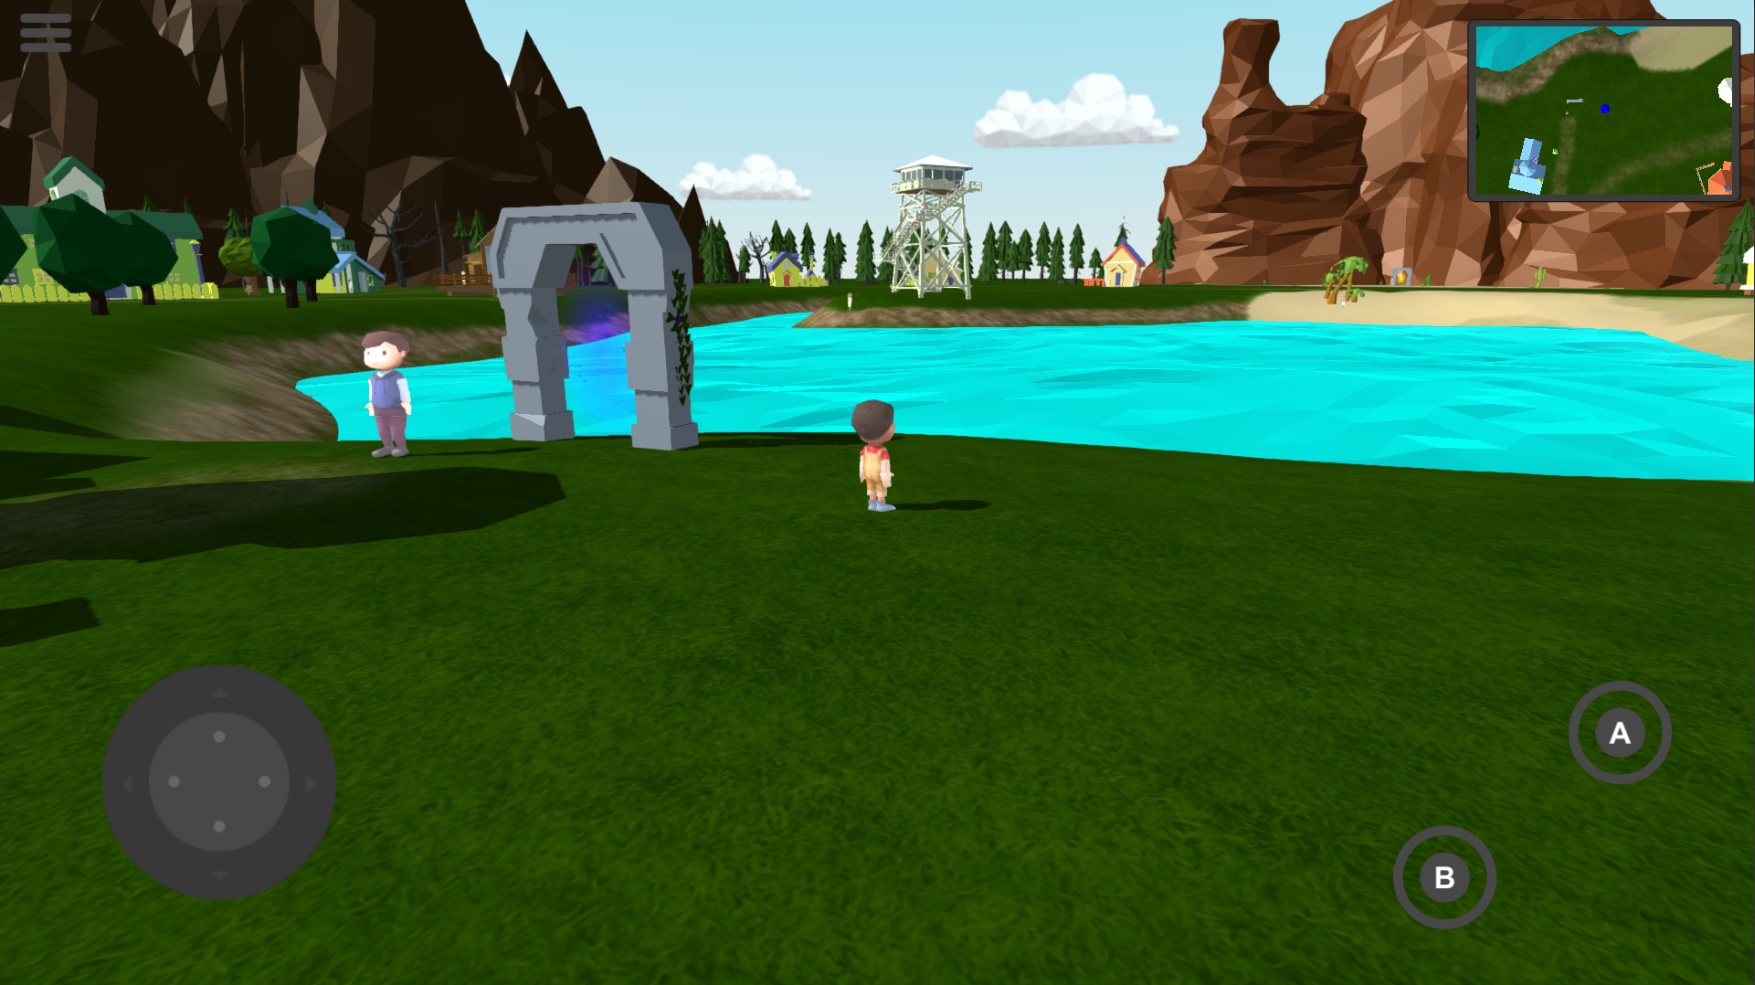
\includegraphics[width=13cm]{pics/alwaysOnUI.png}
			\caption{User Interface: Head-Up Display}
		\end{figure}
	
		\begin{figure}[htbp]
			\centering 
			\label{userInterfaces}
			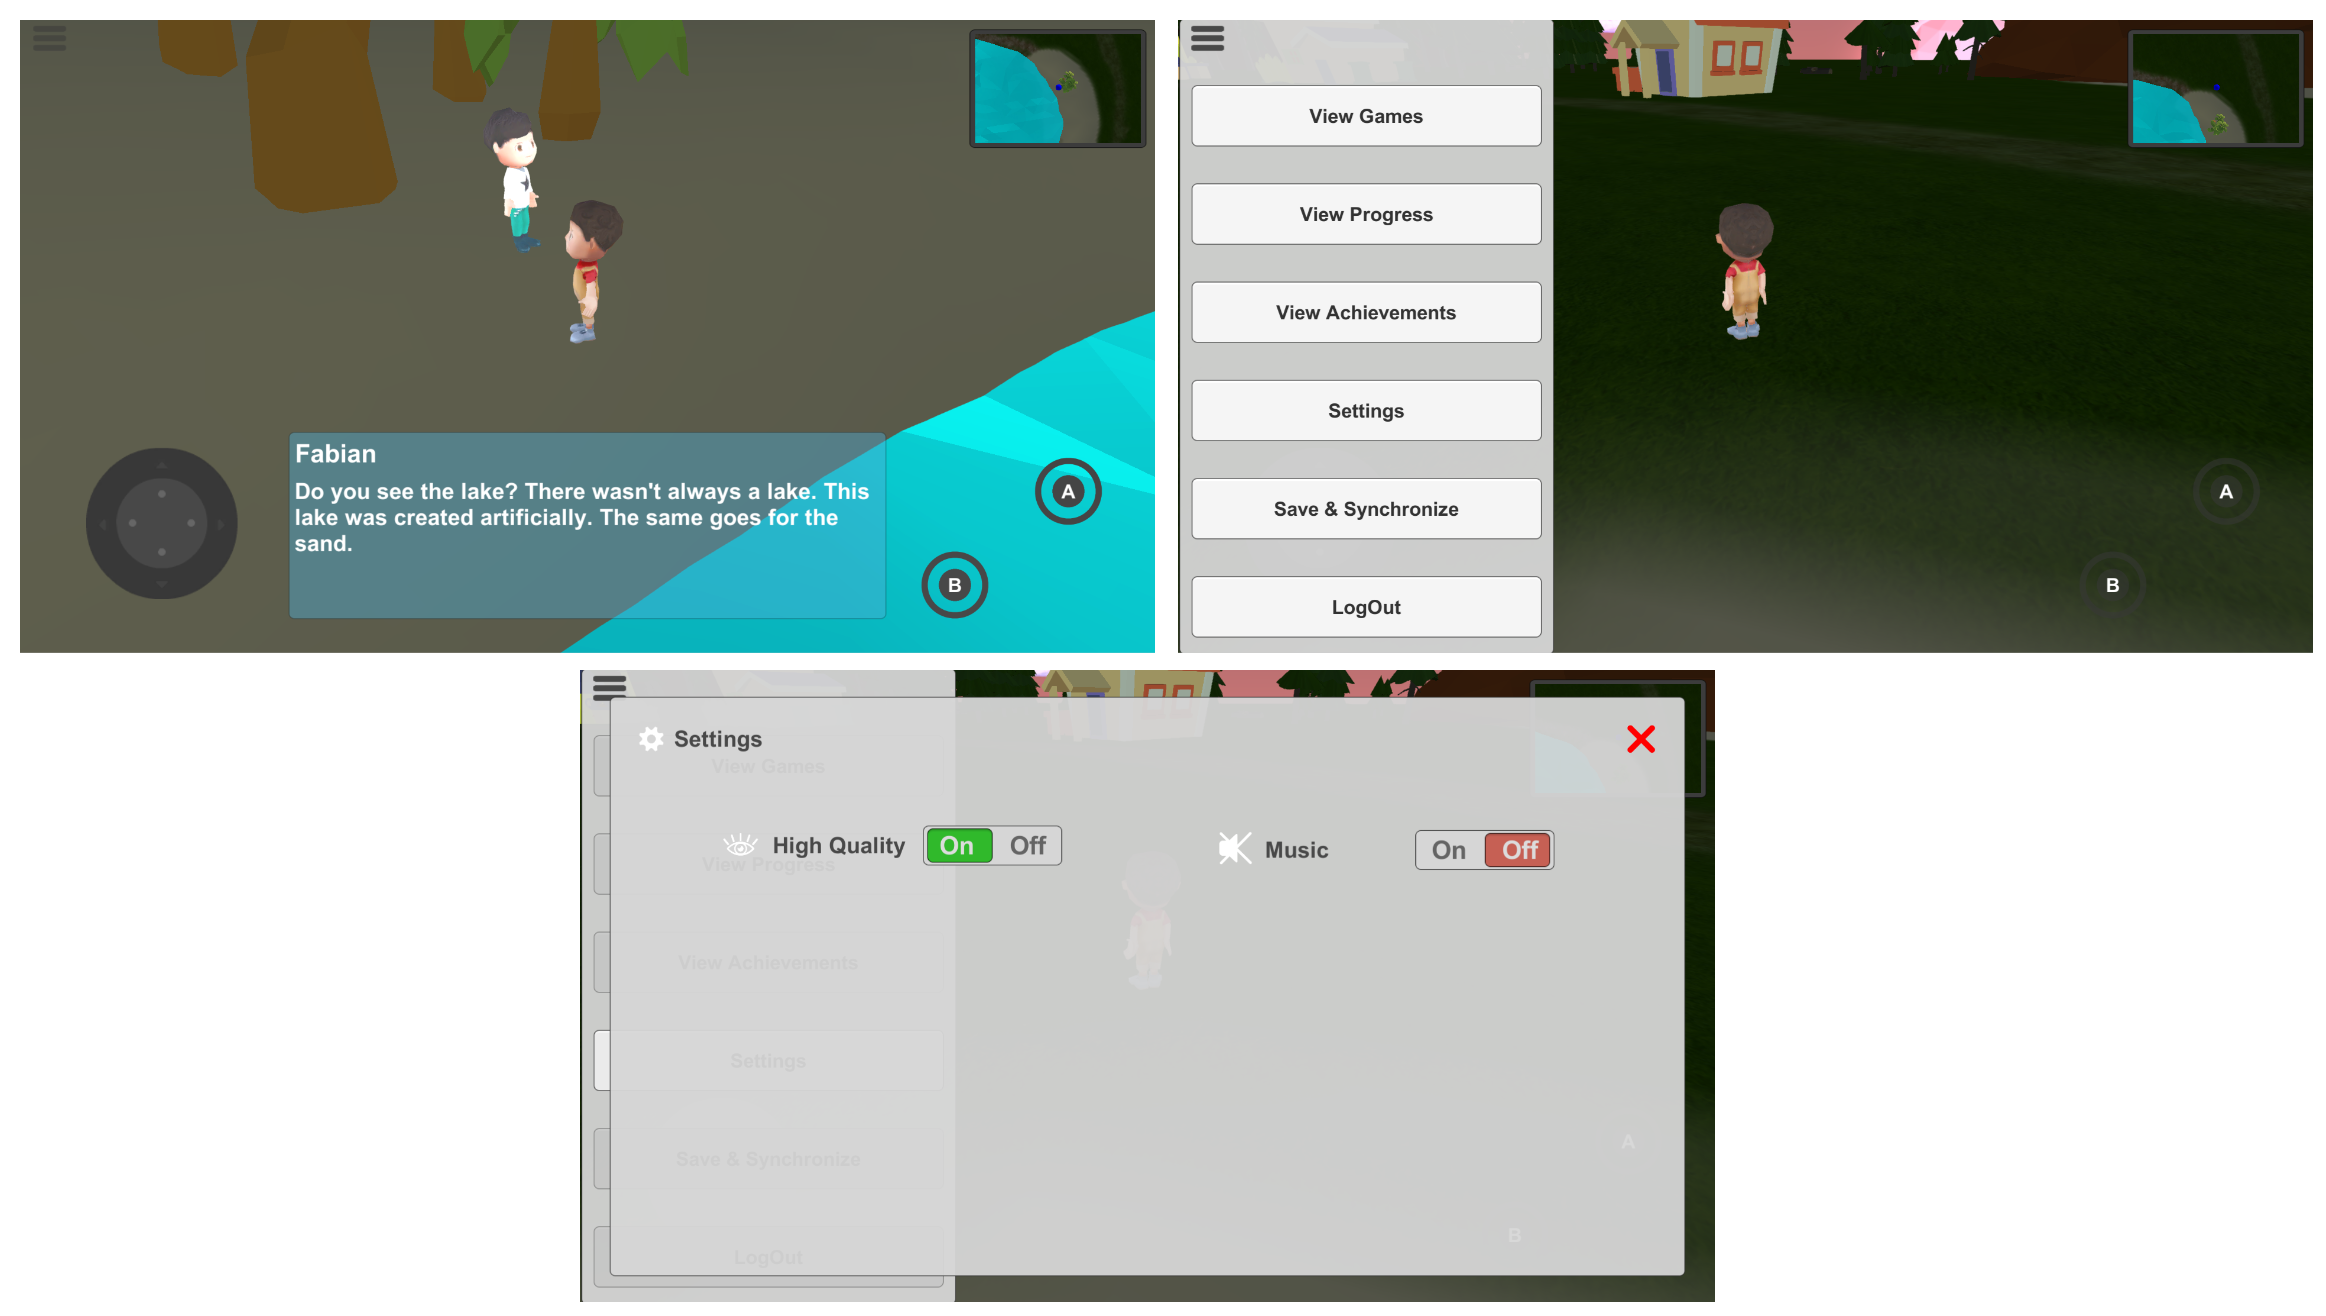
\includegraphics[width=\textwidth]{pics/userInterface.png}
			\caption{User Interfaces: Kommunikation, Menu und Einstellungen-Fenster}
		\end{figure}
	
		Menu fenster bildet die erste Dialogebene nach der Startebene. Nach diesem gibt es noch eine weitere Ebene. dieser Dialog dient zum Abbrechen, warnt vor bevorstehenden Aktionen. Die maximale Dialogebene ist also 2. 

		\begin{figure}[htbp]
			\centering 
			\label{RegisterUI}
			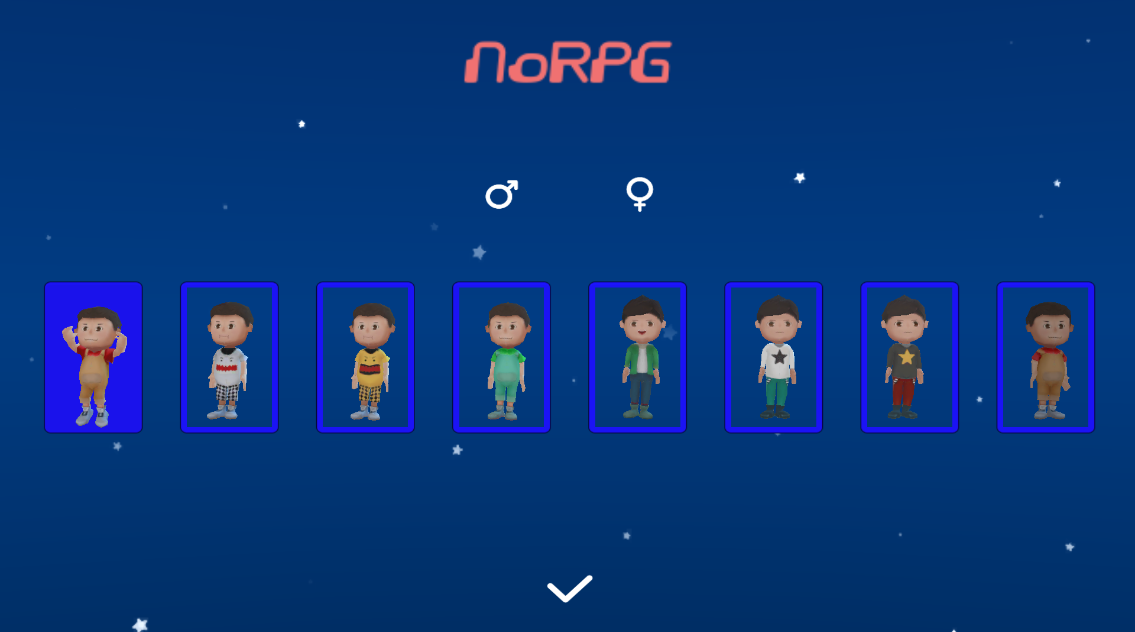
\includegraphics[width=13cm]{pics/RegisterUI.png}
			\caption{User Interface: Registrierung}
		\end{figure}

	
	\subsection{Usability Test}
		EIn Usability Test wird durchgeführt, um die Gebrauchstauglichkeit einer Software oder Hardware mit den potenziellen Benutzern zu überprüfen. Usability wird durch die Attribute Erlernbarkeit, Effizienz, Einprägsamkeit, Fehlerrate und Zufriedenheit\footnote{Vgl. Nielsen \cite{NielsenUI} Seite 26} beschrieben. Die Anwendung sollte leicht zu erlernen sein, damit der Benutzer schnell anfangen kann, seine Aufgaben zu erfüllen. Dazu zählt beispielsweise die Steuerung. Eine einfache Steuerung ist essentiell, damit der Benutzer sich intuitiv im Spiel bewegen kann und es somit keine Umstellung entspricht. Zudem sollte das System effizient zu bedienen sein, so dass, sobald der Benutzer das System gelernt hat, ein hohes Maß an Produktivität möglich ist. Das System sollte allerdings auch leicht zu merken sein, so dass der Gelegenheitsbenutzer in der Lage ist, nach einer gewissen Zeit ohne Verwendung der Anwendung, in das Spiel zurückzukehren, ohne alles nochmals neu lernen zu müssen. Da Fehler sehr frustrierend für den Benutzer sein können, sollte das System eine geringe Fehlerquote haben, so dass Benutzer bei der Verwendung des Systems nur wenige Fehler machen. Der letzte Punkt beschreibt den gesamten Eindruck\footnote{Vgl. Nielsen \cite{NielsenUI} Seite 27ff.}.
		
		Es wird zwischen Formativer und Summativer Usability Test unterschieden. Foramtive Tests werden während der Entwicklung durchgeführt. Das Aufgabe ist es ein spezielles Problem bzw. Ziel zu testen. Es handelt sich um eine kleine Studie für schnelles Feedback die wiederholt werden kann. Der Summativer Test findet nach der Entwicklung statt, bevor das fertige Produkt ausgeliefert wird. Dabei handelt es sich um eine umfangreiche Studie, die alle Funktionen der Benutzeroberfläche bewertet.
		
		Ein Usabilty Test kann in verschiedenen Testumgebungen durchgeführt werden. Es wird zwischen einem Labortest, Feldtest und Remotetest unterschieden. Bei einem Raumtest handelt es sich entweder um ein Usability Labor, welches extra für Usability Tests verwendet wird, oder um einen allgemein nutzbaren Raum. Die potenziellen Tester werden eingeladen und führen die Auswertung in diesem Raum durch. Zu den Basisutensilien in einem Usability Labor gehört neben Nahrung und Verpflegung die notwendige Hardware, sowie eine Möglichkeit die Auswertung auszufüllen. Der Feldtest oder auch Mobiler Test kann potentiell überall durchgeführt werden, sei es beim Kunden, in einem öffentlichen Gebäude oder in einem Café. Der Vorteil im Vergleich zu einem Labortest ist, dass es sich um eine reale Umgebung mit echten Lichtverhältnissen handelt. Der Benutzer ist in seiner gewohnten Umgebung. Bei der letzten Möglichkeit ist der Benutzer und Moderator örtlich voneinander getrennt. Der Remotetest kann Synchron, indem der Moderator und die Teilnehmer per Audio- oder Videokonferenz verbunden sind, oder Asynchron stattfinden. Der wesentliche Vorteil ist, dass dadurch potenziell mehr Testpersonen teilnehmen.
		
		Für das Testen von NoRPG wurde sich für einen summativen Remotetest entschieden. Es handelt sich um einen summativen Test, da es am Ende der Entwicklung durchgeführt wurde. Es wurde sich für einen Remotetest entschieden, da eine mobile Anwendung am besten auf dem eigenen Smartphone getestet werden kann. Es würde sich auch dafür Feldtest eignen, allerdings müsste ein Moderator bei den Testpersonen sein muss. Jedoch ist dies in dem Umfang dieser Projektarbeit nicht möglich. Aber es wurde auch ab und an eine Art Feldtest bei einigen Benutzern durchgeführt, da Kinder vielleicht nicht alleine 
		
		Für das Usability Test wurde ein Formular für die Tester erstellt. Dieses beinhaltet genau alle Information und Schritte die notwendig sind um die Funktionen, die verschiedene UI Elemente hervorbringen, zu testen und anschließend evaluieren zu können.
	
		Zu erst wurden Benutzerprofile erstellt: Benutzer Kinder, alter - aber auch Jugendliche und Erwachsene, daher bei der Evaluation keine Testgruppe eingeschränkt - allerdings ist es wichtig Feedback von Kindern zu erhalten.
		
		Szenarien 
		
		Umfang 
		
		Zeitraum 
	
		TEstutensilien: Prerelease version der APp und eigene Software + Umfrage mit Anleitung
